\documentclass[12pt, twoside]{article}
\documentclass[12pt, twoside]{article}
\usepackage[letterpaper, margin=1in, headsep=0.2in]{geometry}
\setlength{\headheight}{0.6in}
%\usepackage[english]{babel}
\usepackage[utf8]{inputenc}
\usepackage{microtype}
\usepackage{amsmath}
\usepackage{amssymb}
%\usepackage{amsfonts}
\usepackage{siunitx} %units in math. eg 20\milli\meter
\usepackage{yhmath} % for arcs, overparenth command
\usepackage{tikz} %graphics
\usetikzlibrary{quotes, angles}
\usepackage{graphicx} %consider setting \graphicspath{{images/}}
\usepackage{parskip} %no paragraph indent
\usepackage{enumitem}
\usepackage{multicol}
\usepackage{venndiagram}

\usepackage{fancyhdr}
\pagestyle{fancy}
\fancyhf{}
\renewcommand{\headrulewidth}{0pt} % disable the underline of the header
\raggedbottom
\hfuzz=2mm %suppresses overfull box warnings

\usepackage{hyperref}
\usepackage{siunitx}

\title{IB Mathematics}
\author{Chris Huson}
\date{May 2024}

\fancyhead[LE]{\thepage}
\fancyhead[RO]{\thepage \\ Name: \hspace{1cm} \,\\}
\fancyhead[LO]{BECA/Huson/Algebra II 4: Exponential functions \& Rational Exponents \\* 3 May 2024}

\begin{document}

\subsubsection*{4.15 PreExam: Exponential Functions}
Construct an exponential function symbolically given a description of the relationship \hfill F.LE.2.ii

\begin{enumerate}
\item A colony of insects grows exponentially with a growth factor of $3$ each day. By what growth factor does the population change each 12 hours? Express your answer two ways: as a radical and a fractional exponent. \vspace{2cm}
\item A bacteria population, in thousands, is represented by the function $B(t)=100 \times 1.15^t$, where $t$ is the time in hours.
\begin{enumerate}
    \item What is the initial number of bacteria? \vspace{1cm}
    \item What is the growth factor per hour? \vspace{1cm}
    \item What is the growth factor for ten hours? \vspace{2cm}
    \item What is the population after 10 hours? \vspace{2cm}
\end{enumerate}

\item An investment of \$1,000 doubles in value after 6 years. Write an exponential function $V(t)$ to model the investment value, with $t$ in years. Express your answer two ways: as a radical and a fractional exponent.

\newpage
\item The graph shows the exponential function $\displaystyle f(x)$.
\begin{multicols}{2}
    \begin{enumerate}[itemsep=1cm]
        \item Write down the initial value of the function.
        \item By what factor do the values of $f$ increase each time $x$ increases by 1?
        \item Write an expression for the function $f(x)$.
    \end{enumerate}
    \begin{center}
    \begin{tikzpicture}[x=1cm, y=0.15cm, xscale=2]
        \draw [thin, color=lightgray, xstep=0.5cm,ystep=0.75cm] (0,0) grid (3,40);
        \draw [thick, ->] (0,0) -- (+3.3,0) node [below]{$x$};
        \draw [thick, ->] (0,0) -- (0,43) node [right]{$y$};        
        \foreach \x in {0,0.5,...,3}
            \draw (\x cm,0) -- (\x cm,0) node[below] {$\x$};
        \foreach \y in {0,10,20,...,40}
            \draw[shift={(0,\y)}] (2pt,0pt)--(-2pt,0pt) node[left]{$\y$};
        \draw [thick, ->, smooth,domain=0.:2.6] plot(\x,{10*(1.732^\x)}) node[below right]{$f$};
        \fill (0,10) ellipse [x radius=1pt, y radius=2pt]  node [below right] {$(0,10)$};
        \fill (2,30) ellipse [x radius=1pt, y radius=2pt] node [below right] {$(2,30)$};
    \end{tikzpicture}
    \end{center}
    \end{multicols} \vspace{1cm}

\item A sample of radioactive material has a half-life of 8 years. Initially there are 7.5 grams of the material.
    \begin{enumerate}[itemsep=2cm]
        \item How much of the material remains after 8 years?
        \item How much of the material remains after 4 years?
        \item Write an exponential function $A(t)$ to model the amount of material remaining, with $t$ in years.
    \end{enumerate}

\end{enumerate}
\end{document}